% !TEX program = xelatex
\documentclass[12pt,a4paper]{article}

% ---------- Encoding & Language ----------
\usepackage{fontspec}
\usepackage{polyglossia}
\setmainlanguage{greek}
\setotherlanguage{english}
\setmainfont{Times New Roman}
\newfontfamily\greekfont{Times New Roman}

% ---------- Page layout ----------
\usepackage[a4paper,margin=2.5cm]{geometry}
\usepackage{setspace}
\setstretch{1.15}
\usepackage{parskip} % μικρά κενά αντί για εσοχές

% ---------- Figures / Graphics ----------
\usepackage{graphicx}
\usepackage{subcaption}
\usepackage{float}
\usepackage{booktabs}
\usepackage{multirow}
\usepackage{enumitem}
\setlist{nosep}

% ---------- Code & listings ----------
\usepackage{listings}
\lstset{
  basicstyle=\ttfamily\small,
  frame=single,
  breaklines=true,
  tabsize=2,
  showstringspaces=false,
  literate={~}{{\textasciitilde}}1
}

% ---------- Hyperlinks ----------
\usepackage[hidelinks]{hyperref}

% ---------- TikZ UML ----------
\usepackage{tikz}
\usetikzlibrary{arrows.meta,positioning,fit}
\usepackage{tikz-uml}

% ---------- Bibliography (single-file via filecontents*) ----------
\usepackage{csquotes}
\usepackage[backend=biber,style=ieee]{biblatex}
\begin{filecontents*}{references.bib}
@article{wolf2018scanpy,
  title={Scanpy: large-scale single-cell gene expression data analysis},
  author={Wolf, F Alexander and Angerer, Philipp and Theis, Fabian J},
  journal={Genome Biology},
  year={2018},
  volume={19}, number={1}, pages={15}
}
@inproceedings{mcinnes2018umap,
  title={{UMAP}: Uniform Manifold Approximation and Projection for Dimension Reduction},
  author={McInnes, Leland and Healy, John and Melville, James},
  booktitle={arXiv preprint arXiv:1802.03426},
  year={2018}
}
@article{traag2019leiden,
  title={From Louvain to Leiden: guaranteeing well-connected communities},
  author={Traag, Vincent A and Waltman, Ludo and van Eck, Nees Jan},
  journal={Scientific Reports},
  year={2019},
  volume={9}, number={1}, pages={5233}
}
@misc{streamlit,
  title={Streamlit — The fastest way to build data apps},
  howpublished={\url{https://streamlit.io}},
  note={Accessed 2025-08-31}
}
\end{filecontents*}
\addbibresource{references.bib}

% ---------- Title ----------
\title{\textbf{Διαδραστική Εφαρμογή Streamlit για Ανάλυση scRNA\nobreakdash-seq: Σχεδιασμός, Υλοποίηση και Παράδοση με Docker}}
\author{Ονοματεπώνυμο Φοιτητή \\ Τμήμα/Πανεπιστήμιο \\ Ημερομηνία: 31 Αυγούστου 2025}
\date{}

\begin{document}
\maketitle

\begin{abstract}
Παρουσιάζουμε μια διαδραστική εφαρμογή \textit{Streamlit} για ανάλυση μονοκυτταρικών δεδομένων RNA\nobreakdash-seq (scRNA\nobreakdash-seq) που υλοποιεί τυπικό pipeline με \textit{Scanpy} \cite{wolf2018scanpy}: ποιότητα (QC), κανονικοποίηση, επιλογή υψηλής διακύμανσης γονιδίων, \textit{PCA}, γράφος γειτόνων, ενσωμάτωση με \textit{UMAP} \cite{mcinnes2018umap} και ομαδοποίηση με \textit{Leiden} \cite{traag2019leiden}. Η εφαρμογή δέχεται αρχεία \texttt{.mtx/tsv} ή \texttt{.h5ad}, προσφέρει οπτικοποιήσεις (UMAP, violin plots, heatmaps) και εξαγωγή αποτελεσμάτων. Το παρόν κείμενο περιγράφει: (α) τον σχεδιασμό, (β) UML διαγράμματα αρχιτεκτονικής και χρήσης, (γ) τεχνική ανάλυση υλοποίησης, (δ) βασικές οπτικοποιήσεις, και (ε) dockerization για αναπαραγωγιμότητα.
\end{abstract}

\section{Εισαγωγή}
Η ανάλυση scRNA\nobreakdash-seq απαιτεί επαναλήψιμα και διαδραστικά εργαλεία που διευκολύνουν την εξερεύνηση των δεδομένων και την τεκμηρίωση αποφάσεων παραμετροποίησης. Στόχος της παρούσας εργασίας είναι η ανάπτυξη ενός \textit{Streamlit} web app \cite{streamlit} που τυποποιεί τα βασικά βήματα ενός pipeline \cite{wolf2018scanpy} και παρέχει οπτικοποιήσεις για ποιοτικό έλεγχο και βιολογική ερμηνεία.

\paragraph{Συνεισφορές} (i) Ενιαίο UI για φόρτωση \texttt{MatrixMarket} (\texttt{.mtx} + \texttt{barcodes.tsv} + \texttt{features.tsv}) ή \texttt{.h5ad}. (ii) Παραμετρικό preprocessing. (iii) Αυτόματη παραγωγή UMAP/Leiden και βασικών QC plots. (iv) Docker image για εύκολη εκτέλεση.

\section{Σχεδιασμός της Υλοποίησης}
Η αρχιτεκτονική διαχωρίζει \textbf{λογική ανάλυσης} (\texttt{src/}) από το \textbf{UI} (\texttt{app.py, pages/}). Το \texttt{ScanpyAdapter} εγκιβωτίζει τις κλήσεις στη βιβλιοθήκη, ενώ το \texttt{Pipeline} ενορχηστρώνει τα βήματα.

\subsection{UML Class Diagram}
\begin{figure}[H]
  \centering
  \begin{tikzpicture}[scale=0.9, every node/.style={transform shape}]
    % Classes
    \umlclass[x=0,y=0]{DataLoader}{
      - input\_paths : dict\\
      - adata : AnnData
    }{
      + from\_mtx() : AnnData\\
      + from\_h5ad() : AnnData
    }
    \umlclass[x=6.2,y=0]{Preprocessor}{
      - min\_genes : int\\
      - min\_cells : int
    }{
      + filter() : AnnData\\
      + normalize\_log1p() : AnnData\\
      + select\_hvg(n) : AnnData
    }
    \umlclass[x=12.6,y=0]{Analyzer}{
      - n\_pcs : int
    }{
      + pca() : AnnData\\
      + neighbors() : AnnData\\
      + umap() : AnnData\\
      + leiden() : AnnData
    }
    \umlclass[x=6.2,y=-5]{Visualizer}{
      ~ backend : str
    }{
      + qc\_violin() : Figure\\
      + umap() : Figure\\
      + heatmap() : Figure
    }
    \umlclass[x=0,y=-5]{ScanpyAdapter}{}{
      + call(fn, **kwargs)
    }
    \umlclass[x=12.6,y=-5]{Pipeline}{
      - loader : DataLoader\\
      - pre : Preprocessor\\
      - an : Analyzer\\
      - viz : Visualizer
    }{
      + run(params) : AnnData
    }
    % Relations
    \umluniassoc{DataLoader}{ScanpyAdapter}
    \umluniassoc{Preprocessor}{ScanpyAdapter}
    \umluniassoc{Analyzer}{ScanpyAdapter}
    \umluniassoc{Visualizer}{ScanpyAdapter}
    \umluniassoc{Pipeline}{DataLoader}
    \umluniassoc{Pipeline}{Preprocessor}
    \umluniassoc{Pipeline}{Analyzer}
    \umluniassoc{Pipeline}{Visualizer}
  \end{tikzpicture}
  \caption{UML Class Diagram της εφαρμογής.}
  \label{fig:class}
\end{figure}

\subsection{UML Use Case Diagram}
\begin{figure}[H]
  \centering
  \begin{tikzpicture}[scale=0.95, every node/.style={transform shape}]
    % Actor
    \umlactor[x=0,y=0]{Ερευνητής}
    % System boundary
    \node[draw,rounded corners,minimum width=10cm, minimum height=6cm, right=2.5cm of Ερευνητής] (sys) {\textbf{scRNA-seq Streamlit App}};
    % Use cases
    \umlsimpleusecase[x=7,y=2.0,name=uc1]{Φόρτωση Δεδομένων}
    \umlsimpleusecase[x=7,y=1.0,name=uc2]{Παραμετροποίηση Preprocessing}
    \umlsimpleusecase[x=7,y=0.0,name=uc3]{Εκτέλεση Ανάλυσης}
    \umlsimpleusecase[x=7,y=-1.0,name=uc4]{Οπτικοποιήσεις (UMAP/QC)}
    \umlsimpleusecase[x=7,y=-2.0,name=uc5]{Εξαγωγή Αποτελεσμάτων}
    \umlsimpleusecase[x=7,y=-3.0,name=uc6]{Εκτέλεση με Docker}
    % Associations
    \umlassoc{Ερευνητής}{uc1}
    \umlassoc{Ερευνητής}{uc2}
    \umlassoc{Ερευνητής}{uc3}
    \umlassoc{Ερευνητής}{uc4}
    \umlassoc{Ερευνητής}{uc5}
    \umlassoc{Ερευνητής}{uc6}
  \end{tikzpicture}
  \caption{UML Use Case Diagram.}
  \label{fig:usecase}
\end{figure}

\section{Ανάλυση Υλοποίησης με Τεχνικές Λεπτομέρειες}
\subsection{Ροή Pipeline}
Η ροή υλοποιείται σε διακριτές φάσεις:\vspace{2pt}
\begin{enumerate}
  \item \textbf{Φόρτωση}: \texttt{.mtx + barcodes.tsv + features.tsv} ή \texttt{.h5ad} σε αντικείμενο \texttt{AnnData}.
  \item \textbf{QC/Φιλτράρισμα}: κατώφλια \texttt{min\_genes}, \texttt{min\_cells}, προαιρετικά αφαίρεση μιτοχονδριακών.
  \item \textbf{Κανονικοποίηση και Log1p}, επιλογή \textit{HVGs}.
  \item \textbf{PCA} και \textbf{γράφος kNN}, \textbf{UMAP} και \textbf{Leiden}.
  \item \textbf{Οπτικοποιήσεις} και \textbf{εξαγωγή} \texttt{.h5ad}/εικόνων.
\end{enumerate}

\subsection{Ενδεικτικός Κώδικας (Scanpy)}
\begin{lstlisting}[language=Python, caption={Ενδεικτική ακολουθία επεξεργασίας με Scanpy.}]
import scanpy as sc

def run_pipeline(adata, min_genes=200, min_cells=3, n_top_genes=2000, n_pcs=30, res=1.0):
    sc.pp.filter_cells(adata, min_genes=min_genes)
    sc.pp.filter_genes(adata, min_cells=min_cells)
    adata.var['mt'] = adata.var_names.str.upper().str.startswith('MT-')
    sc.pp.calculate_qc_metrics(adata, qc_vars=['mt'], inplace=True)

    sc.pp.normalize_total(adata, target_sum=1e4)
    sc.pp.log1p(adata)
    sc.pp.highly_variable_genes(adata, n_top_genes=n_top_genes, subset=True)

    sc.pp.scale(adata, max_value=10)
    sc.tl.pca(adata)
    sc.pp.neighbors(adata, n_pcs=n_pcs)
    sc.tl.umap(adata)
    sc.tl.leiden(adata, resolution=res)
    return adata
\end{lstlisting}

\subsection{Θέματα Πρακτικής Υλοποίησης}
\begin{itemize}
  \item \textbf{Μεγάλα uploads}: στο Streamlit ρυθμίζουμε μέγιστο μέγεθος αρχείου με \texttt{.streamlit/config.toml}:
\begin{lstlisting}[language=]
[server]
maxUploadSize = 2000  # MB
\end{lstlisting}
  \item \textbf{Αλλαγή API}: προσαρμογή από \texttt{use\_container\_width} σε \texttt{width='stretch'} (deprecation).
  \item \textbf{Εξαρτήσεις}: \texttt{requirements.txt} να περιλαμβάνει τουλάχιστον: \texttt{scanpy, anndata, hdf5plugin, matplotlib, plotly, umap-learn, igraph, leidenalg, streamlit}.
\end{itemize}

\section{Οπτικοποιήσεις Αποτελεσμάτων}
Ενδεικτικά παρουσιάζονται τα κυριότερα διαγράμματα. Αντικαταστήστε τα αρχεία με τα δικά σας στιγμιότυπα από την εφαρμογή (φάκελος \texttt{figs/}).

\begin{figure}[H]
  \centering
  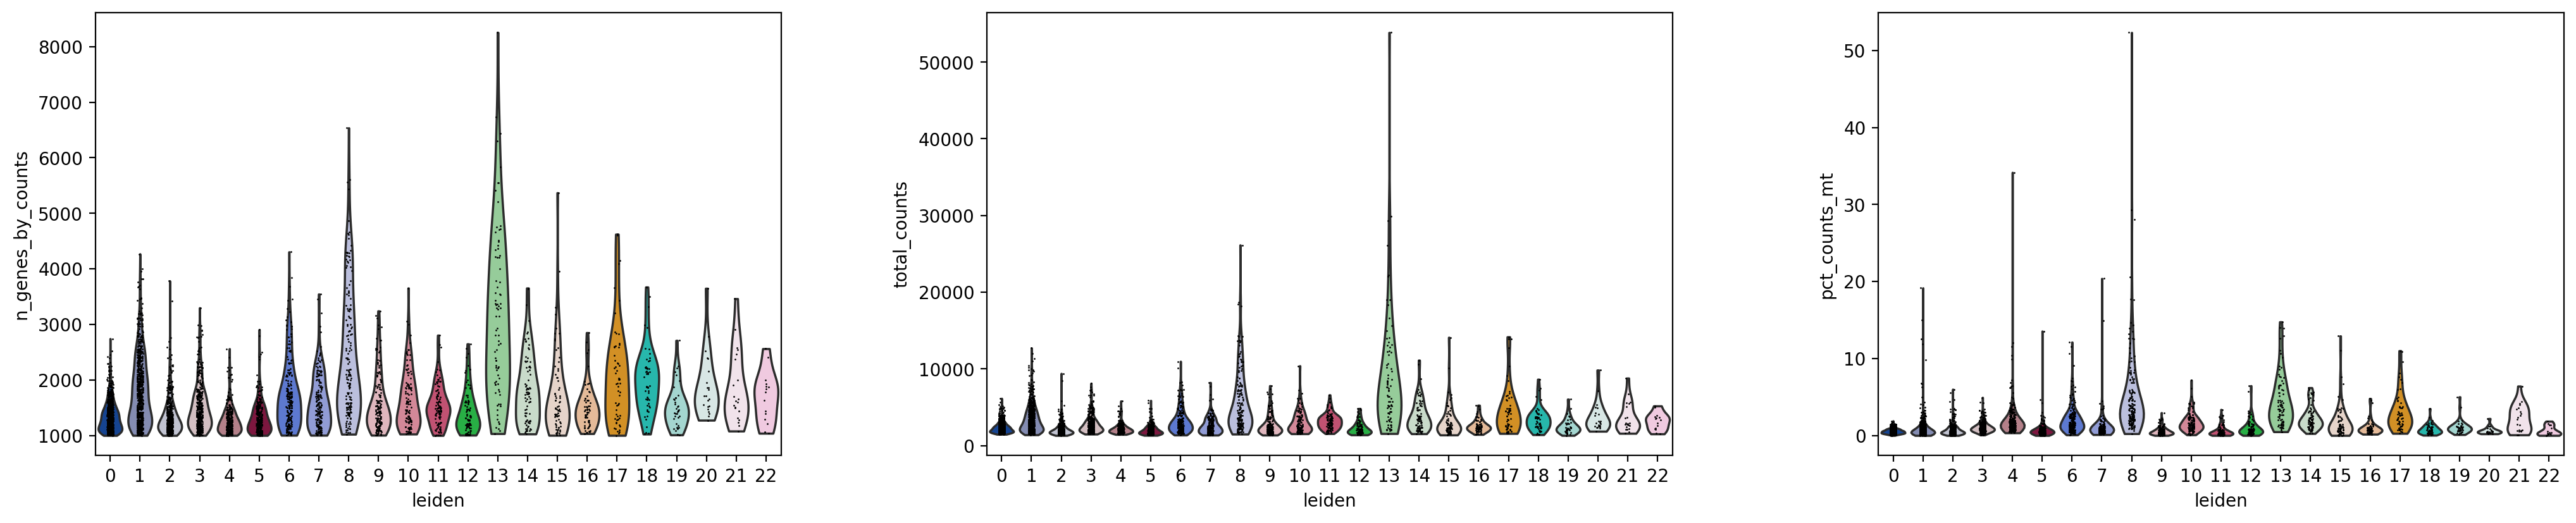
\includegraphics[width=0.8\linewidth]{figs/qc_violin.png}
  \caption{QC violin plots (genes/cell, counts/cell, ποσοστό μιτοχονδριακών).}
  \label{fig:qc}
\end{figure}

\begin{figure}[H]
  \centering
  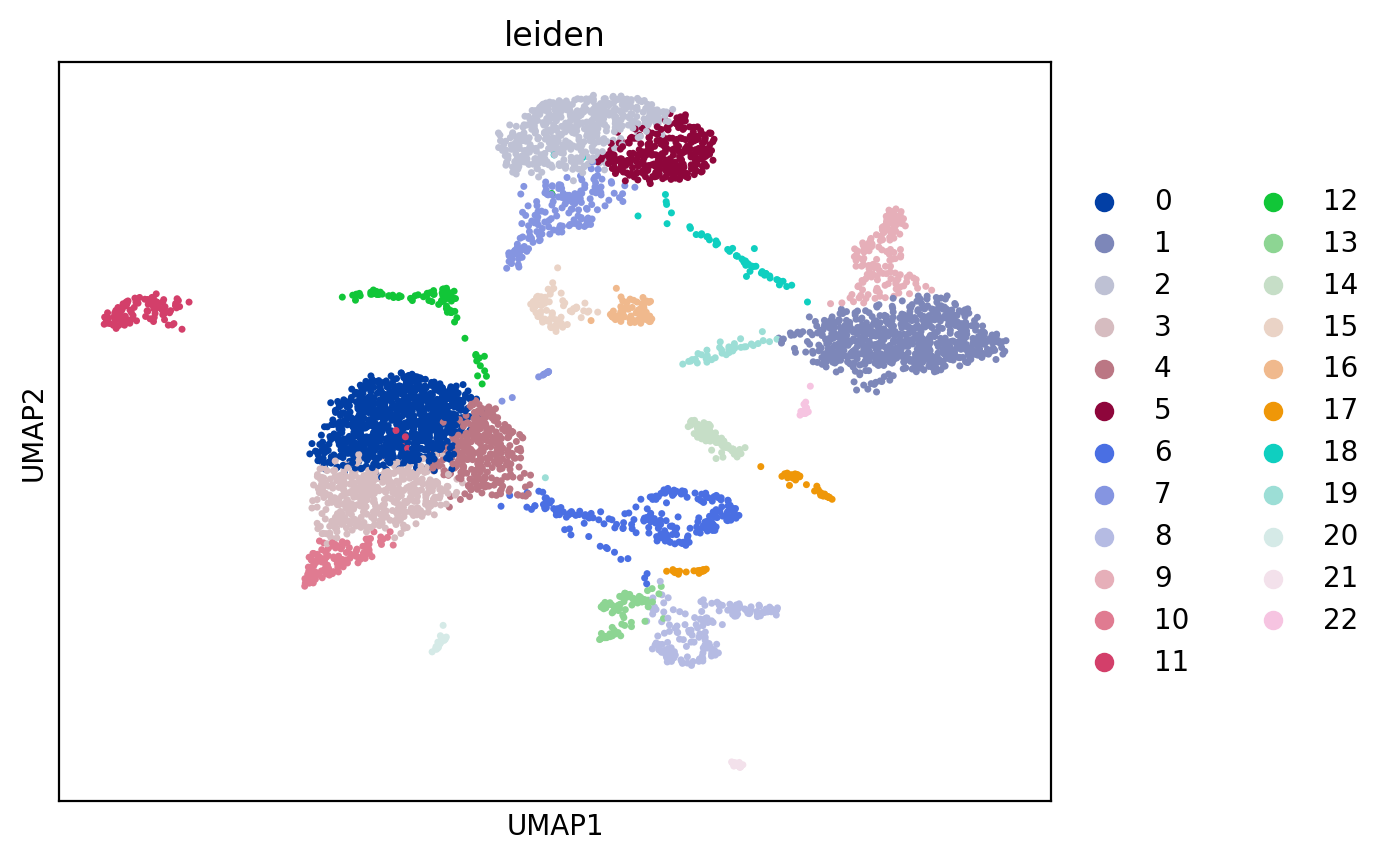
\includegraphics[width=0.8\linewidth]{figs/umap.png}
  \caption{UMAP ενσωμάτωση, χρωματισμός κατά κλάστερ (Leiden).}
  \label{fig:umap}
\end{figure}

\begin{figure}[H]
  \centering
  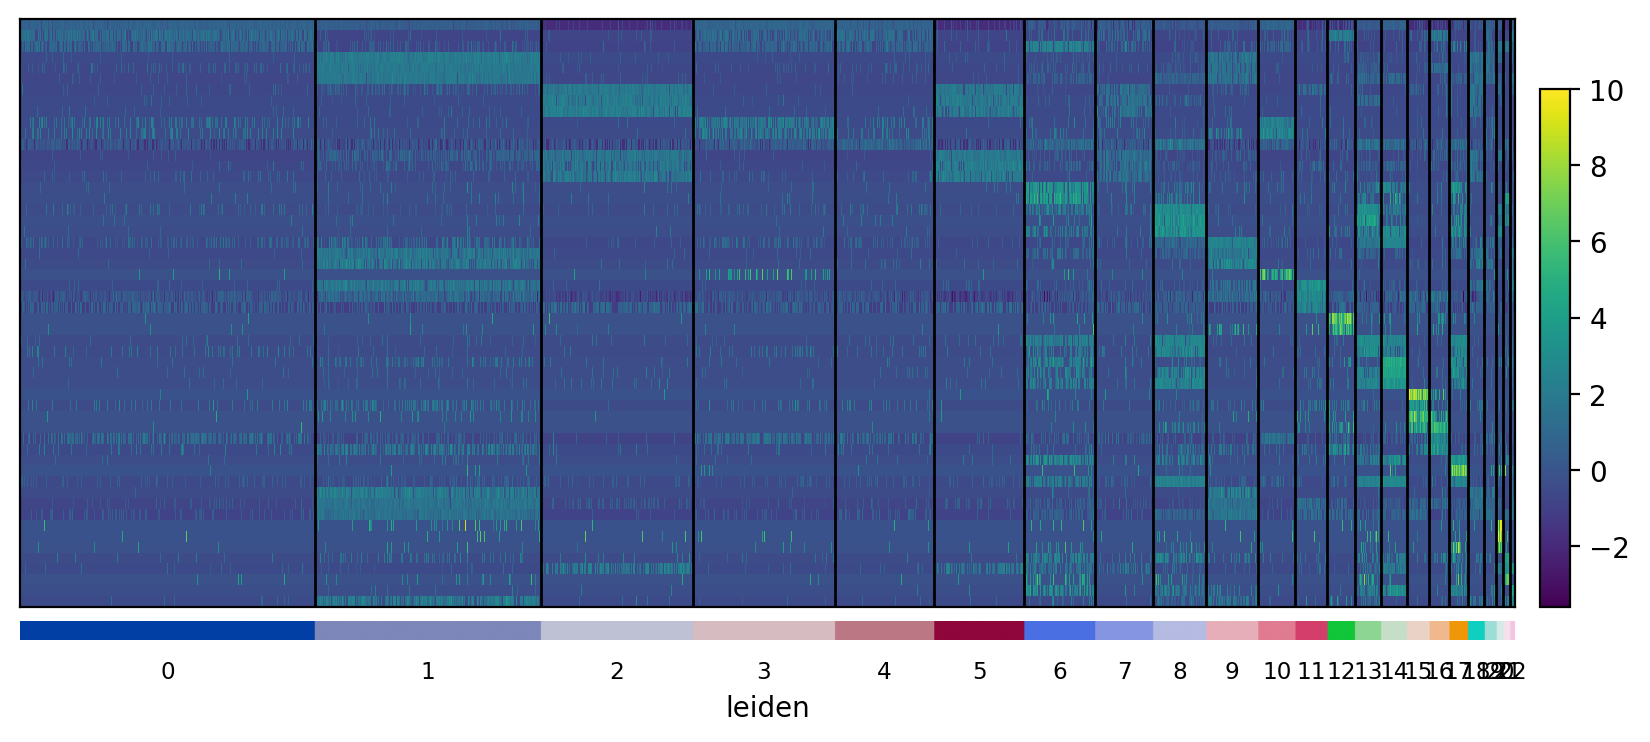
\includegraphics[width=0.8\linewidth]{figs/markers_heatmap.png}
  \caption{Heatmap εκφράσεων επιλεγμένων marker genes ανά κλάστερ.}
  \label{fig:heatmap}
\end{figure}

\section{Dockerization της Εφαρμογής}
\subsection{Dockerfile}
\begin{lstlisting}[language=Dockerfile]
# Dockerfile
FROM python:3.11-slim

# Βασικά εργαλεία για builds
RUN apt-get update && apt-get install -y --no-install-recommends \
    build-essential \
    && rm -rf /var/lib/apt/lists/*

WORKDIR /app
COPY requirements.txt ./
RUN pip install --no-cache-dir -r requirements.txt

COPY . .

# Streamlit ρυθμίσεις παραγωγής
ENV STREAMLIT_SERVER_HEADLESS=true \
    STREAMLIT_SERVER_PORT=8501 \
    STREAMLIT_BROWSER_GATHER_USAGE_STATS=false

EXPOSE 8501
CMD ["streamlit", "run", "app.py"]
\end{lstlisting}

\subsection{Build \\& Run}
\begin{lstlisting}[language=bash]
# Build
docker build -t tl-vol2-scrna-app:latest .

# Run (localhost:8501)
docker run --rm -p 8501:8501 -v %cd%/data:/app/data tl-vol2-scrna-app:latest
\end{lstlisting}

\subsection{Συζήτηση}
Το image πακετάρει όλες τις εξαρτήσεις για αναπαραγωγιμότητα. Η χαρτογράφηση καταλόγου \texttt{data/} επιτρέπει επεξεργασία μεγάλων αρχείων εκτός image. Προαιρετικά multi-stage build για μικρότερο μέγεθος.

\section{Συμπεράσματα}
Παρουσιάστηκε μια ολοκληρωμένη ροή ανάλυσης scRNA\nobreakdash-seq μέσω \textit{Streamlit}, με σαφή διαχωρισμό ευθυνών σε επίπεδο κλάσεων, διαδραστικές οπτικοποιήσεις και πακετάρισμα σε Docker. Μελλοντικά βήματα περιλαμβάνουν ενσωμάτωση αποαναμεμίξεων παρτίδων (\textit{batch correction}) και export notebooks από τις επιλογές χρήστη.

\printbibliography

\end{document}
